%%%%%%%%%%%%%%%%%%%%%%%% ExtendedAbstract.tex %%%%%%%%%%%%%%%%%%%%%%%%
%                                                                    %
%  Template for the 10-page extended abstract to be submitted for    %
%  the MSc degree conferral at Instituto Superior Tecnico.           %
%                                                                    %
%  Author:                                                           %
%                                                                    %
%       Andre C. Marta                                               %
%       Area Cientifica de Mecanica Aplicada e Aeroespacial          %
%       Departamento de Engenharia Mecanica                          %
%       Instituto Superior Tecnico                                   %
%       Av. Rovisco Pais                                             %
%       1049-001 Lisboa                                              %
%       Portugal                                                     %
%       Tel: +351 21 841 9466                                        %
%                        3466 (extension)                            %
%       Email: andre.marta@ist.utl.pt                                %
%                                                                    %
%  Created:       Dec  2, 2011                                       %
%  Last Modified: Dec 27, 2011                                       %
%%%%%%%%%%%%%%%%%%%%%%%%%%%%%%%%%%%%%%%%%%%%%%%%%%%%%%%%%%%%%%%%%%%%%%
% This document uses the LaTeX class file "article.cls"              %
%%%%%%%%%%%%%%%%%%%%%%%%%%%%%%%%%%%%%%%%%%%%%%%%%%%%%%%%%%%%%%%%%%%%%%
\documentclass[10pt,a4paper,twocolumn]{article}

%%%%%%%%%%%%%%%%%%%%%%%%%%%%%%%%%%%%%%%%%%%%%%%%%%%%%%%%%%%%%%%%%%%%%%
% Document preamble
%%%%%%%%%%%%%%%%%%%%%%%%%%%%%%%%%%%%%%%%%%%%%%%%%%%%%%%%%%%%%%%%%%%%%%

%% Builds upon the graphics  package, providing a key-value interface
%% for optional arguments to the \includegraphics command that go far
%% beyone what the graphics package offers.
%% http://www.ctan.org/tex-archive/help/Catalogue/entries/graphicx.html
%% if you use PostScript figures in your article
%% use the graphics package for simple commands
%% \usepackage{graphics}
%% or use the graphicx package for more complicated commands
%% \usepackage{graphicx}
%% or use the epsfig package if you prefer to use the old commands
%% \usepackage{epsfig}
\usepackage{graphicx} % Enhanced LaTeX Graphics

% Multiple figures
\usepackage{subfigure} % subcaptions for subfigures
\usepackage{subfigmat} % matrices of similar subfigures

% Declaring new column types
% 'dcolumn' package defines D to be a column specifier with
% three arguments: D{<sep.tex>}{<sep.dvi>}{<decimal places>}
%                  D{<sep.tex>}{<sep.dvi>}{<left digit places>.<right digit places>}
\usepackage{dcolumn}           % decimal-aligned tabular math columns
% d takes a single argument specifying the number of decimal places, e.g., d{2}
% or the number of digits to the left and right of the seperator, e.g., d{3.2}
\newcolumntype{.}   {D{.}{.}{-1}} % column alignedd on the point separator '.'
\newcolumntype{d}[1]{D{.}{.}{#1}} % column centered on the point separator '.'
\newcolumntype{e}   {D{E}{E}{-1}} % column centered on the exponent 'E'
\newcolumntype{E}[1]{D{E}{E}{#1}} % column centered on the exponent 'E'

%% American Mathematical Society (AMS) plain Tex macros
%%
%% The amsmath package is the principal package in the AMS-LaTeX distribution
%% http://www.ctan.org/tex-archive/help/Catalogue/entries/amsmath.html
\usepackage{amsmath}
%%
%% The amsfonts package provides extended TeX fonts
%% http://www.ctan.org/tex-archive/help/Catalogue/entries/amsfonts.html
\usepackage{amsfonts}
%% The amssymb package provides various useful mathematical symbols
\usepackage{amssymb}
%%
%% The amsthm package provides extended theorem environments
%% http://www.ctan.org/tex-archive/help/Catalogue/entries/amsthm.html
\usepackage{amsthm}

%% Improves the interface for defining floating objects such as figures and tables.
%% The package also provides the H float modifier option of the obsolete here package.
%% http://www.ctan.org/tex-archive/help/Catalogue/entries/float.html
\usepackage{float}

%% Control sectional headers. 
%% http://www.ctan.org/tex-archive/help/Catalogue/entries/sectsty.html
\usepackage{sectsty}
%%
%% Redefine the font size of the 'section' and 'subsection' headings
\newcommand{\myFontSize}{\fontsize{10}{0}\selectfont}
\sectionfont{\myFontSize}       % 10pt, Bold face (default)
\subsectionfont{\rm\myFontSize} % 10pt, Plain face

%% Select alternative section titles.
%% http://www.ctan.org/tex-archive/help/Catalogue/entries/titlesec.html
\usepackage{titlesec}
%%
%% Left indent, before and after spacing
%% (The starred version kills the indentation of the paragraph following the title)
\titlespacing*{\section}{0pt}{10pt}{0pt}
\titlespacing*{\subsection}{0pt}{10pt}{0pt}

%% Section numbers with trailing dots. 
%% http://www.ctan.org/tex-archive/help/Catalogue/entries/secdot.html
\usepackage{secdot}

%% Hyperlinks and cross-references
%% http://www.ctan.org/tex-archive/help/Catalogue/entries/hyperref.html
\usepackage{hyperref}

%% TikZ for drawing diagrams and flowcharts
\usepackage{tikz}
\usetikzlibrary{positioning, shapes.geometric, arrows.meta}

%%
%% Also put a dot after the subsection number
\sectiondot{subsection}
%% Set a space between dot and heading text
\sectionpunct{section}{. }    % By default, \sectiondot places a \quad
\sectionpunct{subsection}{. } % after the number

% These are exact settings for a A4 page with top margin of
% 25 mm, bottom margin of 30 mm, left and right margins of 25 mm,
% printable area 242 X 160 mm.

\setlength{\topmargin}{-10.4mm}
\setlength{\headheight}{0.0mm}
\setlength{\headsep}{10.0mm}
\setlength{\textwidth}{160mm}
\setlength{\textheight}{242mm}
\setlength{\oddsidemargin}{0mm}
\setlength{\evensidemargin}{0mm}
\setlength{\marginparwidth}{0mm}
\setlength{\marginparsep}{0mm}

% New command to refer to equations as Eq.(1),Eq.(2),...
\newcommand{\eqnref}[1]{Eq.(\ref{#1})}


  \renewcommand{\figureautorefname}{Figure}%
  \renewcommand{\tableautorefname}{Table}%
  \renewcommand{\chapterautorefname}{Chapter}%
  \renewcommand{\sectionautorefname}{Section}%
  \renewcommand{\subsectionautorefname}{Subsection}%
  \renewcommand{\equationautorefname}{Equation}%

%%%%%%%%%%%%%%%%%%%%%%%%%%%%%%%%%%%%%%%%%%%%%%%%%%%%%%%%%%%%%%%%%%%%%%%%%%%%%%%%%%%%%%%%
% Title, authors and addresses

\title{Measuring the efficiency of Portuguese and Spanish Airports: A two-stage DEA analysis}
\date{October 2025}
\author{Gonçalo Valente Monteiro da Silva \\ goncalovalentesilva@tecnico.ulisboa.pt \\ \\ Instituto Superior T\'{e}cnico, Lisboa, Portugal}

%%%%%%%%%%%%%%%%%%%%%%%%%%%%%%%%%%%%%%%%%%%%%%%%%%%%%%%%%%%%%%%%%%%%%%%%%%%%%%%%%%%%%%%%
\begin{document}

% Begin one column section for title and abstract
%
% http://www.faqs.org/faqs/de-tex-faq/part5/
\twocolumn[
\begin{@twocolumnfalse}
\maketitle

%%%%%%%%%%%%%%%%%%%%%%%%%%%%%%%%%%%%%%%%%%%%%%%%%%%%%%%%%%%%%%%%%%%%%%
% ABSTRACT & KEYWORDS
%%%%%%%%%%%%%%%%%%%%%%%%%%%%%%%%%%%%%%%%%%%%%%%%%%%%%%%%%%%%%%%%%%%%%%
%%%%%%%%%%%%%%%%%%%%%%%%%%%%%%%%%%%%%%%%%%%%%%%%%%%%%%%%%%%%%%%%%%%%%%
%     File: ExtendedAbstract_abstr.tex                               %
%     Tex Master: ExtendedAbstract.tex                               %
%                                                                    %
%     Author: Andre Calado Marta                                     %
%     Last modified : 2 Dez 2011                                     %
%%%%%%%%%%%%%%%%%%%%%%%%%%%%%%%%%%%%%%%%%%%%%%%%%%%%%%%%%%%%%%%%%%%%%%
% The abstract of should have less than 500 words.
% The keywords should be typed here (three to five keywords).
%%%%%%%%%%%%%%%%%%%%%%%%%%%%%%%%%%%%%%%%%%%%%%%%%%%%%%%%%%%%%%%%%%%%%%

%%
%% Abstract
%%
\vspace{-0.42cm}

\begin{abstract}

The liberalization of the air transport market in Europe led to an unprecedented air traffic growth and the
emergence of Low-Cost Carriers (LCCs), which transformed the aviation industry. This
evolution intensified the need for airports to operate efficiently and adapt continuously to changing
market conditions. Additionally, the growing adoption of concession models in airport management
emphasizes the importance of continuous performance evaluation, to provide objective measures of
efficiency to public regulators.
The present dissertation evaluates the performance of 41 Iberian airports from 2016 to 2023 by
combining Data Envelopment Analysis (DEA) with a two-stage truncated regression and applying a bootstrap
procedure for bias correction. Additionally, the Malmquist Productivity Index (MPI) is used to assess
productivity changes over time.
The results reveal a low average efficiency across airports of the Iberian Peninsula (0.522, excluding
COVID-19 years), especially in the Spanish network, and identify the best and worst performing airports.
The truncated regression highlights the importance of rail intermodal terminals on airports, and indicates
that airports located on Islands, those with Military operations, or those with a higher cargo orientation
tend to be more efficient. The MPI allowed to identify the effects of the COVID-19 pandemic on each
component of airport efficiency, while also presented the airports with best and worst efficiency evolution
in the studied period.
\\
%%
%% Keywords (max 5)
%%
\noindent{{\bf Keywords:}} DEA, Truncated Regressions, MPI, Airport Efficiency, Portugal and Spanish Airports   \\

\end{abstract}



% End one column section (begin default two columns)
\end{@twocolumnfalse}
]
%%%%%%%%%%%%%%%%%%%%%%%%%%%%%%%%%%%%%%%%%%%%%%%%%%%%%%%%%%%%%%%%%%%%%%
% INTRODUCTION
%%%%%%%%%%%%%%%%%%%%%%%%%%%%%%%%%%%%%%%%%%%%%%%%%%%%%%%%%%%%%%%%%%%%%%
%%%%%%%%%%%%%%%%%%%%%%%%%%%%%%%%%%%%%%%%%%%%%%%%%%%%%%%%%%%%%%%%%%%%%%
%     File: ExtendedAbstract_intro.tex                               %
%     Tex Master: ExtendedAbstract.tex                               %
%                                                                    %
%     Author: Andre Calado Marta                                     %
%     Last modified : 27 Dez 2011                                    %
%%%%%%%%%%%%%%%%%%%%%%%%%%%%%%%%%%%%%%%%%%%%%%%%%%%%%%%%%%%%%%%%%%%%%%
% State the objectives of the work and provide an adequate background,
% avoiding a detailed literature survey or a summary of the results.
%%%%%%%%%%%%%%%%%%%%%%%%%%%%%%%%%%%%%%%%%%%%%%%%%%%%%%%%%%%%%%%%%%%%%%

\section{Introduction}
\label{sec:intro}

The air transport market has suffered significant transformations over the last decades, driven by the
liberalization of the industry, which started in 1978 when the United States of America (USA) deregulated
its domestic airline market, meaning airlines were free to set their own fares and routes, without federal
control. This new regulatory framework without market entry
barriers and market restrictions, marked the beginning of an era of unprecedented air traffic growth, where the number of passengers in the world increased from 310 million in 1970 to 4.5 billion in 2019 \cite{baltagi1995}\cite{worldevolution}.

Central to this evolution was the emergence and expansion of Low-Cost Carriers (LCCs). Around 2002, less than 10 years after the implementation of the third package of the EU liberalization process, a steep growth of LCCs started, reaching
30.3\% of the market share in 2018, 10 times more than in 2002 \cite{sharelcc}. Initially operating mostly from secondary or regional airports,
LCCs gradually expanded their operations to larger airports, and are now competing directly with legacy
airlines at major airports \cite{jimenez2020}. This strategic shift of LCCs towards larger airports highlights
the dynamic nature of the air transport market and the consequent need of constant benchmarking to evaluate the performance of airports and adapt accordingly to the changing market conditions. This need for performance analysis is further intensified by the increasing trend towards business
models such as privatization and the use of concessions for airport management, as regulation by public
entities and stakeholders requires transparent and objective performance metrics.

 There are two main benchmarking methodologies: Stochastic Frontier Analysis (SFA), a parametric approach, meaning it requires a predefined functional form
for the production function, and the Data Envelopment Analysis (DEA), a non-parametric approach. These methods are commonly applied in a two-stage analysis, where in the first stage the efficiency scores are calculated using SFA or DEA, and then a second stage analysis is performed to identify exogenous factors that influence efficiency.

Motivated by the decision of developing a new airport in Lisbon, the present work aims to benchmark the efficiency of 41 Iberian airports (5 Portuguese and 36 Spanish) from 2016 to
2023 and identify exogenous factors that influence airport efficiency, such as rail intermodal terminals.

In the next section, a literature review is presented. Then, the methodology used in this work is described, followed by the presentation and discussion of the results. Finally, the main conclusions are drawn and public policy reflections are provided.

%%%%%%%%%%%%%%%%%%%%%%%%%%%%%%%%%%%%%%%%%%%%%%%%%%%%%%%%%%%%%%%%%%%%%%
% BACKGROUND
%%%%%%%%%%%%%%%%%%%%%%%%%%%%%%%%%%%%%%%%%%%%%%%%%%%%%%%%%%%%%%%%%%%%%%
%%%%%%%%%%%%%%%%%%%%%%%%%%%%%%%%%%%%%%%%%%%%%%%%%%%%%%%%%%%%%%%%%%%%%%
%     File: ExtendedAbstract_backg.tex                               %
%     Tex Master: ExtendedAbstract.tex                               %
%                                                                    %
%     Author: Andre Calado Marta                                     %
%     Last modified : 27 Dez 2011                                    %
%%%%%%%%%%%%%%%%%%%%%%%%%%%%%%%%%%%%%%%%%%%%%%%%%%%%%%%%%%%%%%%%%%%%%%
% A Theory section should extend, not repeat, the background to the
% article already dealt with in the Introduction and lay the
% foundation for further work.
%%%%%%%%%%%%%%%%%%%%%%%%%%%%%%%%%%%%%%%%%%%%%%%%%%%%%%%%%%%%%%%%%%%%%%

\section{Literature review}
\label{sec:backg}
In this section a review of the main methodologies used in airport benchmarking is presented, as well as the most commonly employed variables.

Spain, having one of the largest airport operator (Aena), is one of the most frequently analyzed countries in the literature. Therefore, a special focus is given to works analyzing Spanish airports.



%%%%%%%%%%%%%%%%%%%%%%%%%%%%%%%%%%%%%%%%%%%%%%%%%%%%%%%%%%%%%%%%%%%%%%
% IMPLEMENTATION
%%%%%%%%%%%%%%%%%%%%%%%%%%%%%%%%%%%%%%%%%%%%%%%%%%%%%%%%%%%%%%%%%%%%%%
%%%%%%%%%%%%%%%%%%%%%%%%%%%%%%%%%%%%%%%%%%%%%%%%%%%%%%%%%%%%%%%%%%%%%%
%     File: ExtendedAbstract_imple.tex                               %
%     Tex Master: ExtendedAbstract.tex                               %
%                                                                    %
%     Author: Andre Calado Marta                                     %
%     Last modified : 27 Dez 2011                                    %
%%%%%%%%%%%%%%%%%%%%%%%%%%%%%%%%%%%%%%%%%%%%%%%%%%%%%%%%%%%%%%%%%%%%%%
% A Calculation section represents a practical development
% from a theoretical basis.
%%%%%%%%%%%%%%%%%%%%%%%%%%%%%%%%%%%%%%%%%%%%%%%%%%%%%%%%%%%%%%%%%%%%%%

\section{Methodology}
\label{sec:imple}
This section outlines the methodology to be applied throughout this study, namely Data Envelopment Analysis (DEA), Truncated Regression, and the Malmquist Productivity Index (MPI). 
\subsection{Data Envelopment Analysis (DEA)}
\label{dea}
DEA is a non-parametric method used to evaluate the efficiency of Decision Making Units (DMUs) that convert inputs into outputs, by comparing each DMU to a best-practice frontier. The calculated efficiency is relative and is
measured by the distance to the frontier, meaning a DMU is efficient if it lies on the frontier, and inefficient if it lies below it. 

DEA models can be oriented in two ways: input or output oriented. In an input-oriented model the focus is on how much the inputs of a DMU can be proportionally reduced, without affecting the outputs
produced. On the other hand, an output-oriented model focuses on increasing output quantities propor-
tionally, while maintaining the same level of inputs \cite{charnes1994}. 

Another important aspect of DEA is the assumption on returns to scale. In this regard there are two
main formulations, the CCR model (Charnes, Cooper, Rhodes) and the BCC model (Banker, Charnes,
Cooper). The first assumes constant returns to scale (CRS), meaning that an increase in inputs will lead to a proportional increase in outputs. The second assumes variable returns to scale (VRS), meaning it separates the inefficiencies due to scale from those due to pure technical inefficiency, and therefore compares DMUs of similar size \cite{banker1984}. 

Even though the CCR model is a valuable measure of overall efficiency, as airports cannot easily adjust their scale, the BCC model is often more appropriate in this context and will, therefore, be the model applied in this work. \eqnref{output_dea} present the formulation for the output-oriented BCC model. \eqnref{eq:bcc_constraints_output} represent the respective constraints . The main difference between the CCR and BCC models is the inclusion of the convexity constraint (i.e., \(\sum_j \lambda_j = 1\)), which ensures that an inefficient DMU is only benchmarked against similar sized DMUs. 

%\begin{center}
%\textbf{Input-oriented BCC Model}
%\end{center}
%\begin{equation}
 %   \label{input_dea}
%min_{\theta,\lambda} \quad \theta
%\end{equation}
%subject to
%\begin{equation}
%\label{eq:bcc_constraints}
%\begin{gathered}
%\sum_j x_{i,j}\lambda_j \leq \theta x_{i,o} \quad \text{for } i=1,%\ldots,m \\
%\sum_j y_{r,j} \lambda_j \geq y_{r,o} \quad \text{for } r=1,\ldots,s \\
%\sum_j \lambda_j = 1 \\
%\lambda_j \geq 0
%\end{gathered}
%\end{equation}

\vspace{0.5cm}
\begin{center}
\textbf{Output-oriented BCC Model}
\end{center}
\begin{equation}
    \label{output_dea}
max_{\phi,\lambda} \quad \phi
\end{equation}
subject to
\begin{equation}
\label{eq:bcc_constraints_output}
\begin{gathered}
\sum_j y_{r,j} \lambda_j \geq \phi y_{r,o} \quad \text{for } r=1,\ldots,s \\
\sum_j x_{i,j}\lambda_j \leq x_{i,o} \quad \text{for } i=1,\ldots,m \\
\sum_j \lambda_j = 1 \\
\lambda_j \geq 0
\end{gathered}
\end{equation}

To obtain the input-oriented version, the function of \eqnref{output_dea} is replaced by \(min_{\theta,\lambda} \quad \theta\), and the two first inequations are reversed, keeping the rest the same.

Having obtained the efficiency scores using both the CCR and BCC models,
it is possible to obtain the scale efficiency (SE) of an airport. SE measures the loss that a DMU suffers
for not operating at optimal scale, and it is calculated as the ratio between the efficiency scores obtained
using CRS and VRS \cite{bogetoft2011}:

\begin{equation}
    \label{eq:scale_efficiency}
SE = \frac{E_{CRS}}{ E_{VRS}}
\end{equation} 

The value of SE, is always between 0 and 1, since the efficiency score obtained using the CCR model is always less than or equal to that obtained using the BCC model. An SE value of 1 indicates that the DMU is operating at optimal scale, while a value less than 1 indicates that it is not.

Analyzing the value of SE does not provide information on the type of scale inefficiency, i.e., whether
the DMU is operating at increasing or decreasing returns to scale. To identify the nature of the returns to
scale, another model as to be used: the non-increasing returns to scale (NIRS) model, which is derived
from the BCC model by replacing the \(\sum_j \lambda_j = 1\) restriction with \(\sum_j \lambda_j \leq 1\) \cite{coelli2005}. \eqnref{eq:rts_definition} summarizes the classification criteria for the different RTS that can be identified
by comparing the models explained above \cite{huguenin2012}.

\begin{equation}
\label{eq:rts_definition}
RTS =
\begin{cases}
IRS, & \text{if } E_{NIRS} \neq E_{VRS} \\
CRS, & \text{if } E_{NIRS} = E_{VRS} = E_{CRS} \\
DRS, & \text{if } E_{NIRS} = E_{VRS} \neq E_{CRS}
\end{cases}
\end{equation}
 
Efficiency scores obtained using DEA can be influenced not only by management decisions and scale
operation conditions, but also by different exogenous factors. Second-stage regressions are usually
applied to identify the effect of these factors, in which the DEA efficiency values obtained in the first
stage are regressed against a set of potential explanatory variables. In this study, a truncated regression
is going to be applied.

\subsection{Truncated Regression} 
\label{truncreg}

Following \cite{simar2007}, a double bootstrapping procedure is applied in the second-stage
truncated regression that is given by:
\begin{equation}
\label{eq:regression}
\hat{\theta_i}=\alpha+\beta Z_i + \varepsilon_i, \quad i=1,\ldots,n   
\end{equation}
where
\begin{equation}
\label{eq:noise}
\varepsilon_i \sim N(0, \sigma_\varepsilon^2), \quad \text{such that} \quad \varepsilon_i \geq 1 - \alpha - Z_i \beta
\end{equation}
which is estimated by maximizing the corresponding likelihood function.

$\hat{\theta_i}$ represents the bias corrected efficiency value of the $n$ DMUs, $\alpha$ a constant term, $\beta$ the vector of
regression coefficients, $Z_i$ a set of explanatory variables used to evaluate the efficiency scores and $\varepsilon_i$ a
random variable accounting for statistical noise. 

In previous efficiency studies employing DEA, a common practice for estimating the model in \eqnref{eq:regression} had been to employ a censored regression (Tobit). However, \cite{simar2007} demonstrated that this approach is inappropriate because efficiency scores are always higher than 0 and below or equal to 1, meaning the data is truncated at this value rather than censored. Consequently, using a censored regression model would lead to a bias in the estimation.

Since the DEA efficiency scores are relative and not absolute, there is a strong statistical depen-
dency between each observation. Therefore, using them directly in a second-stage regression may
violate fundamental assumptions of regression analysis, such as the independence of the dependent
variable. To overcome the above problems, the bootstrap technique is applied. The double bootstrap approach proposed
by \cite{simar2007} enables consistent inference in the second stage regression, by addressing
the dependency problem, while simultaneously correcting for bias and estimating variance and confidence intervals. 
To facilitate the interpretation of the required steps and their sequential order for the implementation
of algorithm 2 of \cite{simar2007}, \figref{fig:simarwilson} provides a flowchart detailing the 7-step procedure.

\begin{figure}[H]
\centering
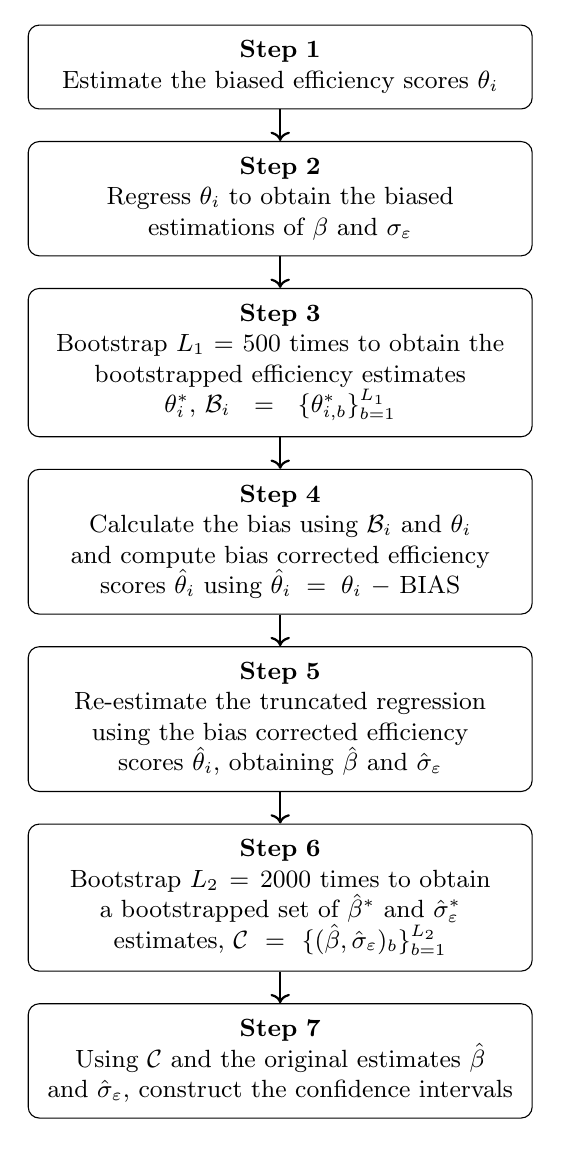
\begin{tikzpicture}[
  node distance=4mm,
  box/.style={
    rectangle, draw, rounded corners,
    text width=60mm, inner sep=2mm, font=\small,
    align=center
  },
  arrow/.style={->, thick}
]
  % Flowchart nodes
  \node[box] (s1) {\textbf{Step 1}\\ Estimate the biased efficiency scores $\theta_i$};
  \node[box, below=of s1] (s2) {\textbf{Step 2}\\ Regress $\theta_i$ to obtain the biased\\ estimations of $\beta$ and $\sigma_\varepsilon$};
  \node[box, below=of s2] (s3) {\textbf{Step 3}\\ Bootstrap $L_1=500$ times to obtain the \\bootstrapped efficiency estimates \\$\theta_i^*$, $\mathcal{B}_i=\{\theta_{i,b}^*\}_{b=1}^{L_1}$};
  \node[box, below=of s3] (s4) {\textbf{Step 4}\\ Calculate the bias using $\mathcal{B}_i$ and $\theta_i$ \\ and compute bias corrected efficiency \\ scores $\hat{\theta}_i$ using $\hat{\theta}_i=\theta_i-\mathrm{BIAS}$};
  \node[box, below=of s4] (s5) {\textbf{Step 5}\\ Re-estimate the truncated regression \\ using the bias corrected efficiency\\ scores $\hat{\theta}_i$, obtaining $\hat{\beta}$ and $\hat{\sigma}_\varepsilon$};
  \node[box, below=of s5] (s6) {\textbf{Step 6}\\ Bootstrap $L_2=2000$ times to obtain\\ a bootstrapped set of $\hat{\beta}^*$ and $\hat{\sigma}_\varepsilon^*$\\ estimates, $\mathcal{C}=\{(\hat{\beta},\hat{\sigma}_\varepsilon)_b\}_{b=1}^{L_2}$};
  \node[box, below=of s6] (s7) {\textbf{Step 7}\\ Using $\mathcal{C}$ and the original estimates $\hat{\beta}$ \\ and $\hat{\sigma}_\varepsilon$, construct the confidence intervals};

  % Flow arrows
  \draw[arrow] (s1) -- (s2);
  \draw[arrow] (s2) -- (s3);
  \draw[arrow] (s3) -- (s4);
  \draw[arrow] (s4) -- (s5);
  \draw[arrow] (s5) -- (s6);
  \draw[arrow] (s6) -- (s7);
\end{tikzpicture}
\caption{Algorithm 2 flowchart based on \cite{simar2007}.}
\label{fig:simarwilson}
\end{figure}

 Although the DEA methodology provides an accurate
static measure of relative efficiency for each year, it does not fully capture how productivity evolves over
time. To address this limitation, the Malmquist Productivity Index (MPI) is also applied, to provide a
dynamic perspective on efficiency changes.

\subsection{Malmquist Productivity Index (MPI)}
\label{mpi}


MPI evaluates the productivity change of a DMU, in our case an airport, by calculating the ratio of
the distance to the frontier in two different time periods, t and t + 1, relative to a common reference
technology. Initially, \cite{caves1982} defined the MPI as follows:

\begin{equation}   
    \label{eq:MI1} 
M_{CCD,\,t} = \frac{D^{t}_{o}\left(x_{t+1}, y_{t+1}\right)}{D^{t}_{o}\left(x_{t}, y_{t}\right)}         
\end{equation}




where $\left(x^{t+1}, y^{t+1}\right)$ represents the input/output combination for the $t+1$ period, and $\left(x^{t}, y^{t}\right)$  for the $t$ period. $D^{t}_{o}\left(x^{t+1}, y^{t+1}\right)$ and $D^{t}_{o}\left(x^{t}, y^{t}\right)$ would then be the distance between the DMU observation in $t+1$ and $t$ periods, respectively, and the best practice frontier in the $t$ period, for airport $o$. 

If one wants to consider the technology from the t + 1 period as the reference, the distance would be measured to the frontier in t + 1 period, meaning $D^{t}_{o}$ would be replaced by $D^{t+1}_{o}$, in the functions of \eqnref{eq:MI1}. To provide a visual illustration of the distance functions defined above, \autoref{fig:fronteiras_malmquist} displays the MPI
distance functions, for $\text{DMU}_\text{X}$, when considering an input orientation.

\begin{figure}[H]
  \centering
  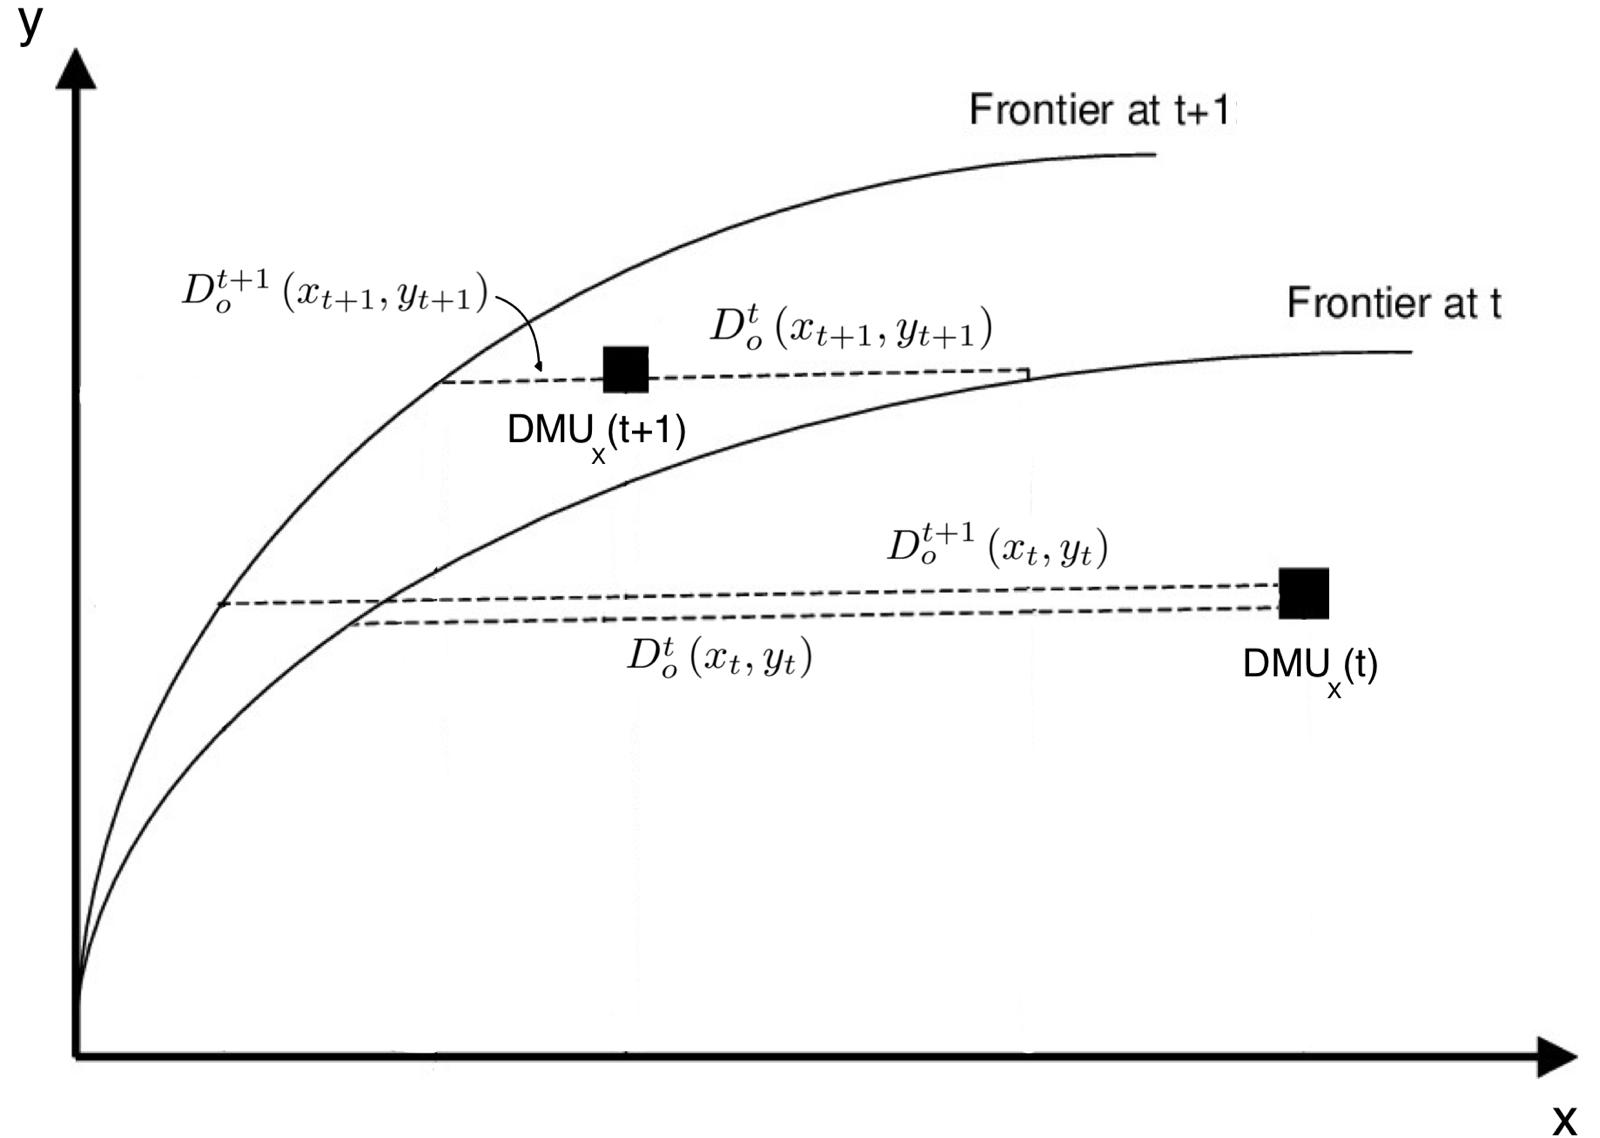
\includegraphics[width=7.5cm]{images/fronteiras_malmquist.jpg}
  \vspace{-0.5cm}
  \caption{Malmquist Productivity Index distance functions for $\text{DMU}_\text{X}$.}
  \label{fig:fronteiras_malmquist}
\end{figure}

In order to avoid the arbitrary selection of a reference technology, \cite{fare1994} specified the
output-based MPI as the geometric mean of the index from \eqnref{eq:MI1}, using both reference technologies, given by:

\begin{equation}
    \label{eq:MI3}
\begin{aligned}
MPI_{o} &= \left[ \left( \frac{D^{t}_{o}(x_{t+1}, y_{t+1})}{D^{t}_{o}(x_{t}, y_{t})} \right) \right. \\
&\quad \left. \left( \frac{D^{t+1}_{o}(x_{t+1}, y_{t+1})}{D^{t+1}_{o}(x_{t}, y_{t})} \right) \right]^{1/2}
\end{aligned}
\end{equation}

According to \cite{fare1994},  an equivalent way of writing the index of \eqnref{eq:MI3} is:


\begin{equation}
\label{eq:MPI}
\begin{aligned}
MPI_{o} &= \underbrace{\frac{D^{t+1}_{o}(x_{t+1}, y_{t+1})}{D^{t}_{o}(x_{t}, y_{t})}}_{\text{Efficiency Change (EC)}} \\
&\times \underbrace{\left[ 
\frac{D^{t}_{o}(x_{t+1}, y_{t+1})}{D^{t+1}_{o}(x_{t+1}, y_{t+1})} 
\times 
\frac{D^{t}_{o}(x_{t}, y_{t})}{D^{t+1}_{o}(x_{t}, y_{t})} 
\right]^{1/2}}_{\text{Technological Change (TC)}}
\end{aligned}
\end{equation}


This formulation decomposes \eqnref{eq:MI3} into two different components: Efficiency change (EC)
and Technological change (TC). The former evaluates if the airport’s efficiency is getting closer or further
away from the best practice frontier (catching-up effect). The latter captures shifts in the frontier itself,
indicating whether there has been technological progress or regress over time.

So far, the analysis has been conducted under constant returns to scale (CRS). However, the first
term (EC) can be further decomposed into Pure Efficiency Change (PEC), associated with VRS, and
Scale Efficiency Change (SEC). To obtain this full decomposition, two additional programming problems are required, namely the
calculation of Dt+1
o
(xt+1, yt+1) and Dt
o(xt, yt) under VRS, which provides the value of PEC and allows
the calculation of SEC, following the definition of \eqnref{eq:scale_efficiency}. 

A $MPI_{o}$ greater than one indicates an improvement in efficiency between periods t and t + 1. The
same interpretation applies to the other all the other components of the MPI. Conversely, a value less
than one indicates a decline in efficiency

%%%%%%%%%%%%%%%%%%%%%%%%%%%%%%%%%%%%%%%%%%%%%%%%%%%%%%%%%%%%%%%%%%%%%%
% RESULTS
%%%%%%%%%%%%%%%%%%%%%%%%%%%%%%%%%%%%%%%%%%%%%%%%%%%%%%%%%%%%%%%%%%%%%%
%%%%%%%%%%%%%%%%%%%%%%%%%%%%%%%%%%%%%%%%%%%%%%%%%%%%%%%%%%%%%%%%%%%%%%
%     File: ExtendedAbstract_resul.tex                               %
%     Tex Master: ExtendedAbstract.tex                               %
%                                                                    %
%     Author: Andre Calado Marta                                     %
%     Last modified : 27 Dez 2011                                    %
%%%%%%%%%%%%%%%%%%%%%%%%%%%%%%%%%%%%%%%%%%%%%%%%%%%%%%%%%%%%%%%%%%%%%%
% Results
% Results should be clear and concise.
% Discussion
% This should explore the significance of the results of the work, not
% repeat them. A combined Results and Discussion section is often
% appropriate. Avoid extensive citations and discussion of published
% literature.
%%%%%%%%%%%%%%%%%%%%%%%%%%%%%%%%%%%%%%%%%%%%%%%%%%%%%%%%%%%%%%%%%%%%%%

\section{Results}
\label{sec:resul}
In this section, the dataset used is described and the results obtained are presented. First, the descriptive statistics are provided, then the DEA scores are obtained, followed by the truncated regression analysis, and finally the Malmquist index results.
\subsection{Descriptive Statistics}
\label{subsec:resul_data}
Our dataset includes 41 Iberian airports, including 5 in Portugal and 36 in Spain, over a period of eight years (2016-2023). Following the airport size definition from \cite{ripoll-zarraga2020}, \figref{fig:mapa} displays a map with the geographical location of the airports and their respective sizes.  

\vspace{-0.25cm}
\begin{figure}[h!]
  \centering
  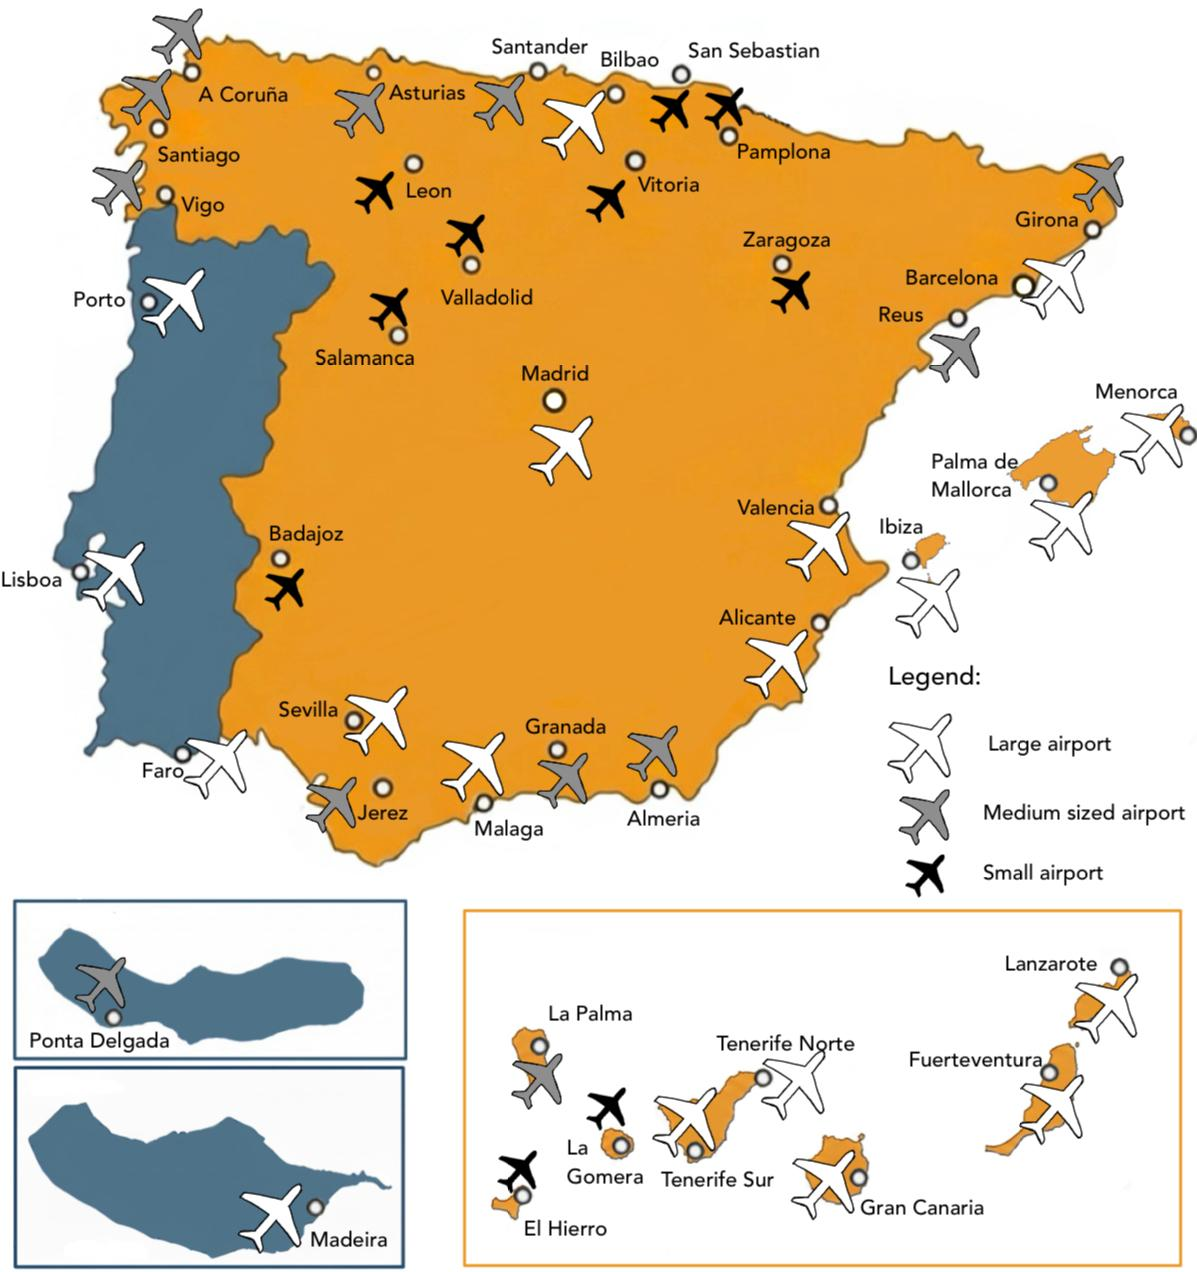
\includegraphics[width=8cm]{images/mapa.jpg}
  \vspace{-0.5cm}
  \caption{Location and size classification of the 41 Iberian airports}
  \label{fig:mapa}
\end{figure}

\vspace{-0.3cm}
DEA models require the identification of the inputs and outputs of the analysis. As DEA is not a
statistical technique, there is no systematic approach for the selection of inputs and outputs, thus the first practical criterion for selecting these
variables is data availability. \tabref{tab:variables} lists these variables
and summarizes their main descriptive statistics, namely the minimum (Min.), maximum (Max.), mean,
and standard deviation (St. Dev.) values.

\clearpage
\begin{table}[h!]
  \begin{center}
    \caption{Summary Statistics for Input and Output Variables (2016–2023)}
    \label{tab:variables}
    \resizebox{\columnwidth}{!}{%
  \begin{tabular}{lcccc}
        \toprule
        \textbf{Variables} & \textbf{Min.} & \textbf{Max.} & \textbf{Mean} & \textbf{St. Dev.} \\
        \midrule
        \multicolumn{5}{l}{\textit{Inputs}} \\
       Employees & 17 & 42,222 & 3,409 & 7,862 \\
         Runway \\Area
    ($m^2$) & 37,500 & 910,020 & 169,293 & 142,191 \\
        Gates & 2 & 238 & 24.8 & 42.4 \\
        \midrule
        \multicolumn{5}{l}{\textit{Outputs}} \\
         Passengers & 2,358 & 61,652,021 & 6,437,865 & 11,112,114 \\
        ATM & 1,086 & 426,324 & 53,780 & 76,780 \\
         Cargo (t) & 0 & 655,586 & 27,546 & 89,429 \\
        \bottomrule
 \end{tabular}%
    }
  \end{center}
\end{table}
  \vspace{-0.5cm}
Even though this selection of input variables does not fully
represent the most common variables in the literature review conducted in \autoref{sec:backg}, due to data availability constraints, it is still in line with the previous literature. It is important to highlight that only physical measures of capital were considered in this analysis, since airport-level financial data stopped being published, following Aena’s partial privatization in 2014.

Regarding the second-stage regression, \tabref{tab:exp_statistics} lists the explanatory variables used in the second-stage regression to explain DEA efficiency scores.

\vspace{-0.2cm}
\begin{table}[h!]
  \begin{center}
        \caption{Summary Statistics for explanatory variables}
    \label{tab:exp_statistics}
    % Define centered column type
   \resizebox{\columnwidth}{!}{%
  \begin{tabular}{lcccc}
        \toprule
        \textbf{Explanatory Variables} & \textbf{Min.} & \textbf{Max.} & \textbf{Mean} & \textbf{St. Dev.} \\
        \midrule
        Island & 0 & 1 & 0.32 & 0.47 \\
        Military & 0 & 1 & 0.27 & 0.44 \\
        Rail existence & 0 & 1 & 0.10 & 0.30 \\
        Share of cargo (\%) & 0 & 89.33 & 4.68 & 15.65 \\
        Share of LCC passengers (\%) & 0 & 96.67 & 49.62 & 26.78 \\
        \bottomrule
  \end{tabular}%
    }
  \end{center}
\end{table}
  
\vspace{-0.5cm}
Island is a binary variable indicating whether an airport is located on an island (Island=1) or the
mainland (Mainland=0). The inclusion of this variable is justified, as 13 out of the 49 airports in the
dataset operate on an island. Military is another binary variable indicating whether there are military
operations at the airport. In the considered dataset, 11 out of the 41 airports operate as mixed civil-military airports.
Share of cargo represents the percentage of cargo in the total WLU and Share of LCC passengers the percentage of low-cost carrier (LCC) passengers in the total
number of passengers. 
Additionally, a novel input in Iberian airport efficiency studies was included: the existence of a railway connection inside the airport. This variable was included to capture the impact of intermodal connectivity on airport efficiency.







\subsection{First-stage: Static DEA scores}
\label{subsec:resul_dea}  
The first stage of the analysis involved calculating the efficiency scores for each airport across the
different years considered. For that, an output oriented DEA model under Variable Returns to Scale
(VRS) was applied.

The choice of output orientation is particularly appropriate in the context of Iberian airports, since
most of the Spanish airports operate with overcapacity, meaning the existing infrastructure is underutilized \cite{nerja2021}. As some of the airport inputs are considered fixed in the short and medium term, airport managers have limited capacity to adjust input levels,
and should, therefore, focus on maximizing their utilization \cite{martin2001}. Regarding the returns to scale, VRS was assumed due to the size differences between the airports considered, as shown in \figref{fig:mapa}. Nonetheless, the CRS
scores were also determined for the calculation of Scale efficiencies. 

\tabref{tab:crs,vrs,scale} presents the DEA bootstrapped results obtained for each airport. It includes the average efficiency scores for Constant Returns to Scale (CRS), Variable Returns to Scale (VRS), and Scale efficiency (Scale) for each airport. It should be noted that the biased scores were also calculated for comparison, even though they are not presented for brevity. Following the definition in \eqnref{eq:rts_definition}, the last column indicates the type of returns to scale (RTS) each airport is operating, which can
be either Increasing Returns to Scale (IRS), Decreasing Returns to Scale (DRS), or Constant Returns to Scale (CRS). As this study analyzes a period of 8 years, different classifications can be obtained in
different years. In \tabref{tab:crs,vrs,scale}, the most common classification will be displayed. In cases where the two
most common classifications are observed the same number of times across the eight-year period, both
classifications are presented.

Analyzing \tabref{tab:crs,vrs,scale}, it is possible to observe that Iberian airports present low values of efficiency,
averaging 0.480 for the bootstrapped VRS model, in the years under
analysis.
When excluding the years 2020 and 2021, due to the COVID-19 pandemic, the average
bootstrapped VRS efficiency increases to 0.522, while the CRS model increases to 0.436. It is also
possible to note that there is no average efficiency score of 1, with a maximum observed
value of 0.823 for Madrid-Barajas airport, meaning none of the considered airports operates in the
frontier. Regarding scale efficiency, the average bootstrapped scale efficiency is 0.854, indicating that
Iberian airports are not operating at their optimal scale.

Regarding the returns to scale (RTS) classification, out of the 41 airports considered, 21 operate
under IRS. This result further confirms the fact that a majority of airports in the Spanish centralized
system are underutilized and have the potential to increase their efficiency by expanding their operation,
as argued by \cite{nerja2021}. On the other hand, a smaller set of 9 airports operate under DRS, meaning
they could improve their efficiency by reducing their operations. Out of the 41 airports, 7 of them obtained
more than one classification. Only 4 airports were classified
with CRS, meaning they operate at their optimal scale. Analyzing the Portuguese airports, it can be
observed that all operate under IRS. 

\vspace{-0.2cm}
%\renewcommand{\arraystretch}{0.9}
\begin{table}[h!]
\centering
\caption{Bootstrapped average CRS, VRS and Scale efficiencies.} 
\vspace{-0.2cm}
\label{tab:crs,vrs,scale}
\resizebox{\columnwidth}{!}{%
\begin{tabular}{lcccc}
  \toprule
  \textbf{Airports} & \textbf{CRS} & \textbf{VRS} & \textbf{Scale} & \textbf{RTS}  \\
  \midrule

% no \endhead here to prevent repeated header

% === Table rows start here ===
A Coruña & 0.323 & 0.343 & 0.941 & IRS\\
A S Madrid-Barajas & 0.568 & 0.823 & 0.693 & DRS\\
Alicante & 0.591 & 0.596 & 0.988 & IRS/DRS \\
Almeria & 0.226 & 0.232 & 0.978 & IRS/CRS\\
Asturias & 0.188 & 0.190 & 0.987 & CRS\\
Badajoz & 0.121 & 0.360 & 0.335 & IRS\\
Barcelona & 0.382 & 0.741 & 0.518 & DRS\\
Bilbao & 0.436 & 0.501 & 0.871 & DRS\\
El Hierro & 0.325 & 0.768 & 0.425 & IRS\\
Faro & 0.514 & 0.551 & 0.928 & IRS\\
FGL Granada & 0.366 & 0.414 & 0.883 & IRS\\
Fuerteventura & 0.353 & 0.370 & 0.952 & DRS\\
Girona & 0.183 & 0.186 & 0.982 & IRS/CRS\\
Gran Canaria & 0.448 & 0.552 & 0.809 & IRS\\
Ibiza & 0.694 & 0.698 & 0.991 & DRS/CRS\\
Jerez & 0.653 & 0.680 & 0.961 & DRS\\
La Gomera & 0.183 & 0.516 & 0.388 & IRS\\
La Palma & 0.276 & 0.288 & 0.959 & IRS\\
Lanzarote & 0.588 & 0.596 & 0.985 & IRS\\
Leon & 0.124 & 0.492 & 0.297 & IRS\\
Lisbon & 0.617 & 0.701 & 0.880 & IRS\\
Madeira & 0.237 & 0.254 & 0.933 & IRS\\
Malaga & 0.522 & 0.583 & 0.883 & DRS\\
Menorca & 0.332 & 0.342 & 0.970 & IRS/DRS\\
Palma De Mallorca & 0.464 & 0.661 & 0.701 & IRS\\
Pamplona & 0.173 & 0.224 & 0.776 & IRS\\
Ponta Delgada & 0.417 & 0.703 & 0.596 & IRS\\
Porto & 0.608 & 0.650 & 0.923 & IRS\\
Reus & 0.262 & 0.262 & 0.999 & IRS/CRS\\
Salamanca & 0.645 & 0.649 & 0.995 & IRS/CRS\\
San Sebastian & 0.128 & 0.148 & 0.866 & IRS\\
Santiago & 0.234 & 0.243 & 0.963 & DRS\\
Santander & 0.191 & 0.193 & 0.992 & CRS\\
Sevilla & 0.534 & 0.564 & 0.946 & DRS\\
Tenerife-Norte & 0.534 & 0.580 & 0.916 & IRS\\
Tenerife-Sur & 0.636 & 0.658 & 0.966 & DRS\\
Valencia & 0.536 & 0.550 & 0.971 & IRS\\
Valladolid & 0.177 & 0.178 & 0.995 & CRS\\
Vigo & 0.168 & 0.168 & 0.997 & CRS\\
Vitoria & 0.563 & 0.694 & 0.820 & IRS\\
Zaragoza & 0.802 & 0.822 & 0.976 & IRS\\
\midrule
Mean & 0.398 & 0.480 & 0.854 & \\
Mean excluding COVID & 0.436 & 0.522 & 0.859 & \\
\# of efficient DMUs & 0 & 0 & 18 & \\
\bottomrule
\end{tabular}%
}
\end{table}

\vspace{-0.2cm}



For a better comparison of the performance of the considered airports, \figref{fig:boxplot} presents a boxplot  
graph displaying the minimum, first quartile, median, third quartile and maximum values of the boot-
strapped VRS efficiency scores, for each airport, over the years considered. For easier interpretation of
the results, a dotted line was added to indicate the average efficiency score of 0.522. Also, the data for
the COVID years (2020 and 2021) was excluded from the boxplot, as they are not representative of the
airports’ normal operation. However, they are still included in the graph and marked by red dots.

Analyzing \figref{fig:boxplot}, and considering the median value of each box, it is possible to observe
that, from the 41 airports, 24 present above average efficiencies, with Madrid-Barajas, Barcelona and
Zaragoza obtaining the highest efficiency scores, while San Sebastian, Valladolid and Vigo being the
least efficient airports. Following the airport size definition presented in \figref{fig:mapa}, 16 of the 24 airports
with above average efficiency are large, while 14 of the 17 below average airports are small or medium
sized. This result suggests that larger airports tend to be more efficient. 

  \vspace{-0.4cm}

\begin{figure}[h!]
  \centering
  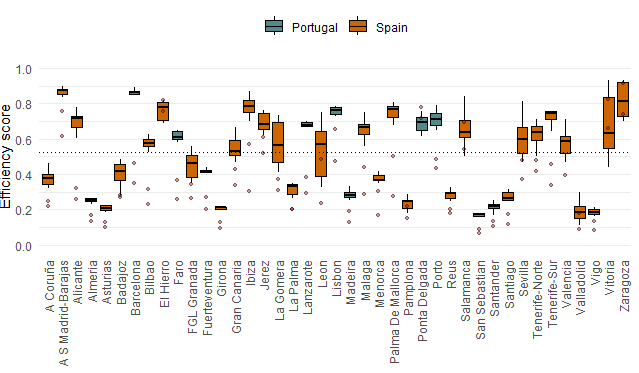
\includegraphics[width=8cm]{images/Rplot01.png}
  \vspace{-0.8cm}
  \caption{Boxplots of the bootstrapped VRS efficiency scores, for each airport.}
  \label{fig:boxplot}
\end{figure}

\vspace{-0.3cm}

Considering the Portuguese airports, only Madeira airport is considered inefficient, with Lisbon being
the most efficient, followed by Porto, Ponta Delgada and Faro. The average efficiency for Portuguese
airports is 0.613, indicating that, over the period and sample considered, they are approximately 20 %
more efficient than the Spanish ones that obtained an average efficiency of 0.510.




\vspace{-0.1cm}
\subsection{Second-stage: Truncated regression }
\label{subsec:resul_trunc}

After computing the DEA efficiency scores in the first stage, a second-stage truncated regression
was conducted to address DEA’s main limitation, which is its inability to explain the effect of some
determinants in the efficiency scores. The regression was applied to the bootstrapped DEA scores, using the explanatory variables described in \tabref{tab:exp_statistics}, under the following model:

\vspace{-0.6cm}
\begin{equation}
    \label{eq:complete_regression}
\begin{aligned}
\theta_{i,t} &= \alpha + \beta_1 \text{Island}_{i} + \beta_2 \text{Military}_{i} + \beta_3 \text{Rail}_{i} \\
&\quad + \beta_4 \text{ShareCargo}_{i,t} + \beta_5 \text{ShareLCC}_{i,t} + \varepsilon_{i,t}
\end{aligned}
\end{equation}

\tabref{tab:regression_results} reports the coefficients and p-values for the variables considered in both the biased and
bootstrapped models. For binary variables, the coefficient represents the estimated change in the effi-
ciency score when the specific variable applies, while for continuous variables, the coefficient reflects
the marginal effect on the efficiency score of a one-unit increase in the corresponding variable \cite{simar2007}.

Analyzing the results, it is possible to observe that the coefficients of the variables are similar across
both models, with the bootstrapped model presenting consistently lower values. Starting by the Island
variable, its coefficient is positive and statistically significant at the 1\% significance level in both models,
indicating that airports located on islands are, on average, 18.58\% and 16.90\% more efficient than
those located on the mainland, respectively. It can also be concluded that the presence of Military operations in the airport contributes positively
on the efficiency, with a coefficient of 8.22\% in the biased model and 6.44\% in the bootstrapped one, with
the former being statistically significant at the 10\% significance level and the latter at the 5\% significance
level.
\begin{table}[h!]
\centering
\caption{Truncated regression results.}
\label{tab:regression_results}
\resizebox{\columnwidth}{!}{%
\begin{tabular}{l D{.}{.}{1.4} D{.}{.}{1.4} c D{.}{.}{1.4} D{.}{.}{1.4}}
    \toprule
\multirow{2}{*}{\textbf{Variable}} &\multicolumn{2}{c}{\textbf{Biased}} & \hspace{0.01cm} & \multicolumn{2}{c}{\textbf{Bootstrapped}} \\
\cmidrule{2-3} \cmidrule{5-6}
 & \multicolumn{1}{l}{\textbf{Coeff.}} & \multicolumn{1}{l}{\textbf{p-value}} && \multicolumn{1}{l}{\textbf{Coeff.}} & \multicolumn{1}{l}{\textbf{p-value}} \\
\midrule
\textit{Constant} & 0.5175 & 0.0000^{***} && 0.2602 & 0.0000^{***} \\ 
Island & 0.1858 & 0.0000^{***} && 0.1690 & 0.0000^{***} \\ 
Military & 0.0822 & 0.0578^{*} && 0.0644 & 0.0210^{**} \\ 
Rail existence & 0.4895 & 0.0000^{***} && 0.3828 & 0.0000^{***} \\ 
Share of cargo & 0.0108 & 0.0000^{***} && 0.0065 & 0.0000^{***} \\ 
Share of LCC & -0.0016 & 0.0234^{**} && 0.0007 & 0.1670 \\ 
\bottomrule
\end{tabular}%
}
\begin{flushleft}
\footnotesize
\textit{Note}: Statistically significant at 1\% $^{***}$, 5\% $^{**}$, or 10\% $^{*}$ level.
\end{flushleft}
\end{table}

\vspace{-0.5cm}
 Regarding the novel explanatory variable in Iberian airport studies, Rail existence, it achieved the
highest coefficient, from all variables and revealed to be statistically significant at the 1\% level, in both
models. An Iberian airport with a conventional rail connection is, on average, 48.95\% more efficient in
the biased model and 38.28\% in the bootstrapped one, respectively, than one without such a connection. Focusing on the effect the share of cargo transport has on airport efficiency, it is possible to observe
that the coefficient is positive and statistically significant at the 1\% significance level in both models,
indicating that a 1\% increase in the share of cargo, in the total WLU, results in an increase in the
efficiency score of 1.08\%, for the biased model, and 0.65\%, for the bootstrapped one. As for the share of LCC passengers, the results were inconclusive. In the biased model, the coefficient was negative and statistically significant at the 5\% significance level, suggesting that a 1\% increase
in the share of LCC passengers would lead to a 0.16\% decrease in the efficiency score. In contrast, in
the bootstrapped model, the coefficient became positive (0.07\%) but was not statistically significant.





\subsection{Dynamic Evolution: Malmquist index}
\label{subsec:resul_malm}
To complement the obtained static DEA scores, the Malmquist Productivity Index
(MPI) was applied to analyze how the productivity of each Iberian airport evolved over the considered
period (2016-2023). The dynamic evaluation that this methodology offers becomes especially important
for a period that includes an external shock as the COVID-19 pandemic, since it allows for a better
understanding of the impact of such events in airport performance, not only in the affected years (in this
case, 2020 and 2021), but also in the subsequent recovery years.

\tabref{tab:malmquist_summary} presents the geometric means of the MPI for the Iberian airports, as well as the four components it can be decomposed into: Technological Change (TECHC), Efficiency Change (EC), which is further divided into Pure Efficiency Change (PEC) and Scale Efficiency Change (SEC). Two additional notes must be done: first, the MPI calculations were made without accounting for the bias present in
the DEA scores, i.e., no bootstrapping technique was applied, as no function in the softwares (RStudio
and Stata) used is readily available. Second, 4 of the initial 41 airports do not present the results of
the decomposition of EC, due to failure in the estimation of PEC (that is obtained by conducting a MPI
analysis under VRS), namely for the airports El Hierro, La Gomera, Leon and Ponta Delgada.


Analyzing \tabref{tab:malmquist_summary}, it is possible to observe that, on average, Iberian airports experienced a productivity growth of 3.82\% over the period considered, with 37 out of the 41 airports showing improvement  (MPI $>$ 1). The main driver of this productivity growth was Efficiency Change (EC), which increased by 3.27\%, while Technological Change (TECHC) contributed with a smaller increase of 0.58\%. This result indicates that most of the productivity growth was due to improvements in how efficiently airports utilized their resources, rather than advancements in technology or infrastructure. An expected result is that the highest values of Technological Change (TECHC) are concentrated in
the largest airports as Madrid-Barajas, Barcelona, Lisbon, Porto and Valencia, with values ranging from
1.0367 to 1.0848. When analyzing the decomposition of EC, it is possible to observe that the average Pure Efficiency
Change (PEC) increased by 2.96\%, while Scale Efficiency Change (SEC) slightly decreased by 0.24\%.
This suggests that most of the efficiency improvements were due to better management and operational
practices, rather than changes in the scale of operations.


The best performing airports in the considered period were Badajoz, Leon and Valencia. The latter
achieved the highest MPI, with a value of 1.1265, indicating a significant productivity growth of 12.65\%.
This growth was mainly driven by a strong increase in EC (8.66\%), with both PEC and SEC contributing
positively to the efficiency change. Leon and Badajoz also showed strong performance, with MPIs of
1.1234 and 1.1119, respectively, driven by improvements in efficiency rather than advancements of the
frontier. Unfortunately, for Leon the decomposition of EC cannot be analyzed but for Badajoz, unlike
Valencia a decrease of 7.87\% in the scale efficiency was registered.
\vspace{-0.2cm}
%\renewcommand{\arraystretch}{0.9}
\begin{table}[h!]
\centering
\caption{Geometric mean of Malmquist Productivity Index (MPI) and its components for each airport} 
\label{tab:malmquist_summary}
\resizebox{\columnwidth}{!}{%
\begin{tabular}{lccccc}
  \toprule
  \textbf{Airport} & \textbf{MPI} & \textbf{TECHC} & \textbf{EC} & \textbf{PEC} & \textbf{SEC} \\
  \midrule
A Coruña & 1.0096 & 0.9863 & 1.0236 & 1.0317 & 0.9922 \\
A S Madrid-Barajas & 1.0486 & 1.0566 & 0.9924 & 1.0000 & 0.9924 \\
Alicante-Elche & 1.0238 & 1.0331 & 0.9910 & 0.9931 & 0.9980 \\
Almería & 1.0007 & 0.9792 & 1.0219 & 1.0277 & 0.9944 \\
Asturias & 1.0660 & 0.9945 & 1.0718 & 1.0819 & 0.9907 \\
Badajoz & 1.1119 & 1.0094 & 1.1016 & 1.1970 & 0.9203 \\
Barcelona & 1.0420 & 1.0848 & 0.9605 & 1.0000 & 0.9605 \\
Bilbao & 1.0173 & 0.9841 & 1.0337 & 1.0118 & 1.0216 \\
El Hierro &1.0462 & 0.9812 & 1.0662 &  &  \\  
Faro & 0.9550 & 0.9920 & 0.9627 & 0.9898 & 0.9726 \\
FGL Granada & 0.9974 & 0.9758 & 1.0221 & 1.0187 & 1.0033 \\
Fuerteventura & 1.0126 & 1.0067 & 1.0059 & 0.9961 & 1.0098 \\
Girona & 1.0006 & 0.9940 & 1.0067 & 1.0054 & 1.0012 \\
Gran Canaria & 1.0459 & 1.0196 & 1.0258 & 1.0196 & 1.0060 \\
Ibiza & 1.0240 & 1.0069 & 1.0170 & 1.0136 & 1.0033 \\
Jerez & 1.0107 & 1.0107 & 1.0000 & 1.0000 & 1.0000 \\
La Gomera &1.1073& 0.9764& 1.1341 &  &  \\ 
La Palma & 1.0282 & 0.9940 & 1.0345 & 1.0334 & 1.0011 \\
Lanzarote & 1.0269 & 1.0079 & 1.0189 & 1.0174 & 1.0014 \\
Leon & 1.1234 & 0.9938 & 1.1305 &  &  \\
Lisbon & 1.0566 & 1.0566 & 1.0000 & 1.0000 & 1.0000 \\
Madeira & 1.0393 & 1.0159 & 1.0230 & 1.0296 & 0.9936 \\
Malaga & 1.0435 & 1.0184 & 1.0247 & 0.9964 & 1.0284 \\
Menorca & 1.0160 & 0.9965 & 1.0196 & 1.0165 & 1.0030 \\
Palma de Mallorca & 1.0253 & 1.0400 & 0.9858 & 0.9976 & 0.9882 \\
Pamplona & 1.0468 & 0.9929 & 1.0543 & 1.0683 & 0.9869 \\
Ponta Delgada & 1.0512& 1.0300 & 1.0205 &  &  \\
Porto & 1.0595 & 1.0595 & 1.0000 & 1.0000 & 1.0000 \\
Reus & 1.0341 & 0.9788 & 1.0565 & 1.0583 & 0.9983 \\
Salamanca & 0.9863 & 0.9829 & 1.0034 & 1.0000 & 1.0034 \\
San Sebastián & 1.0229 & 0.9781 & 1.0459 & 1.0465 & 0.9995 \\
Santiago & 1.0438 & 0.9881 & 1.0564 & 1.0548 & 1.0015 \\
Santander & 1.0557 & 0.9838 & 1.0731 & 1.0855 & 0.9887 \\
Sevilla & 1.0436 & 0.9983 & 1.0454 & 1.0366 & 1.0084 \\
Tenerife Norte & 1.0305 & 1.0214 & 1.0089 & 1.0114 & 0.9975 \\
Tenerife-Sur & 0.9818 & 0.9988 & 0.9830 & 0.9760 & 1.0072 \\
Valencia & 1.1265& 1.0367 & 1.0866 &1.0600 & 1.0251 \\
Valladolid & 1.0799 & 0.9704 & 1.1128 & 1.1165 & 0.9967 \\
Vigo & 1.0230 & 0.9823 & 1.0415 & 1.0446 & 0.9970 \\
Vitoria & 1.1004 & 1.0191 & 1.0797 & 1.0598 & 1.0188 \\
Zaragoza & 1.0031 & 1.0031 & 1.0000 & 1.0000 & 1.0000 \\
 \midrule
 Mean & 1.0382
 & 1.0058  
 & 1.0327
 &1.0296
 & 0.9976
 \\
 \midrule
\end{tabular}%
}
\end{table}
\vspace{-0.2cm}



As already mentioned, 4 of the 41 airports presented a decrease in efficiency, namely Faro, FGL Granada, Salamanca and Tenerife-Sur. Faro had the lowest MPI, with a value of 0.9550, indicating a productivity
decline of 4.50\%. This result is explained by a decrease in TECHC (0.80\%) and EC (3.73\%), with both
PEC and SEC contributing negatively to the EC result. FGL Granada also experienced a
slight decline in productivity, with an MPI of 0.9974, driven by a decrease in TECHC (2.42\%) despite the
increase in EC (2.21\%). Salamanca and Tenerife-Sur had similar MPI results, with values of 0.9863 and
0.9818, respectively. Both airports experienced declines in TECHC (1.71\% and 0.12\%, respectively)
while for EC, Salamanca had a slight increase (0.34\%) and Tenerife-Sur a decrease (1.70\%). Also, both
airports presented an improvement in scale.

To better understand how the MPI changed and what caused its variations along the years, \figref{fig:malmquist}
displays the evolution of the average MPI and its components for each year. The score of each year
represents the change in relation to the previous year. To provide the starting point representation, the
first year 2016, was also added, so all the components under study have a value equal to one in this
year.
\vspace{-0.5cm}
\begin{figure}[H]
  \centering
  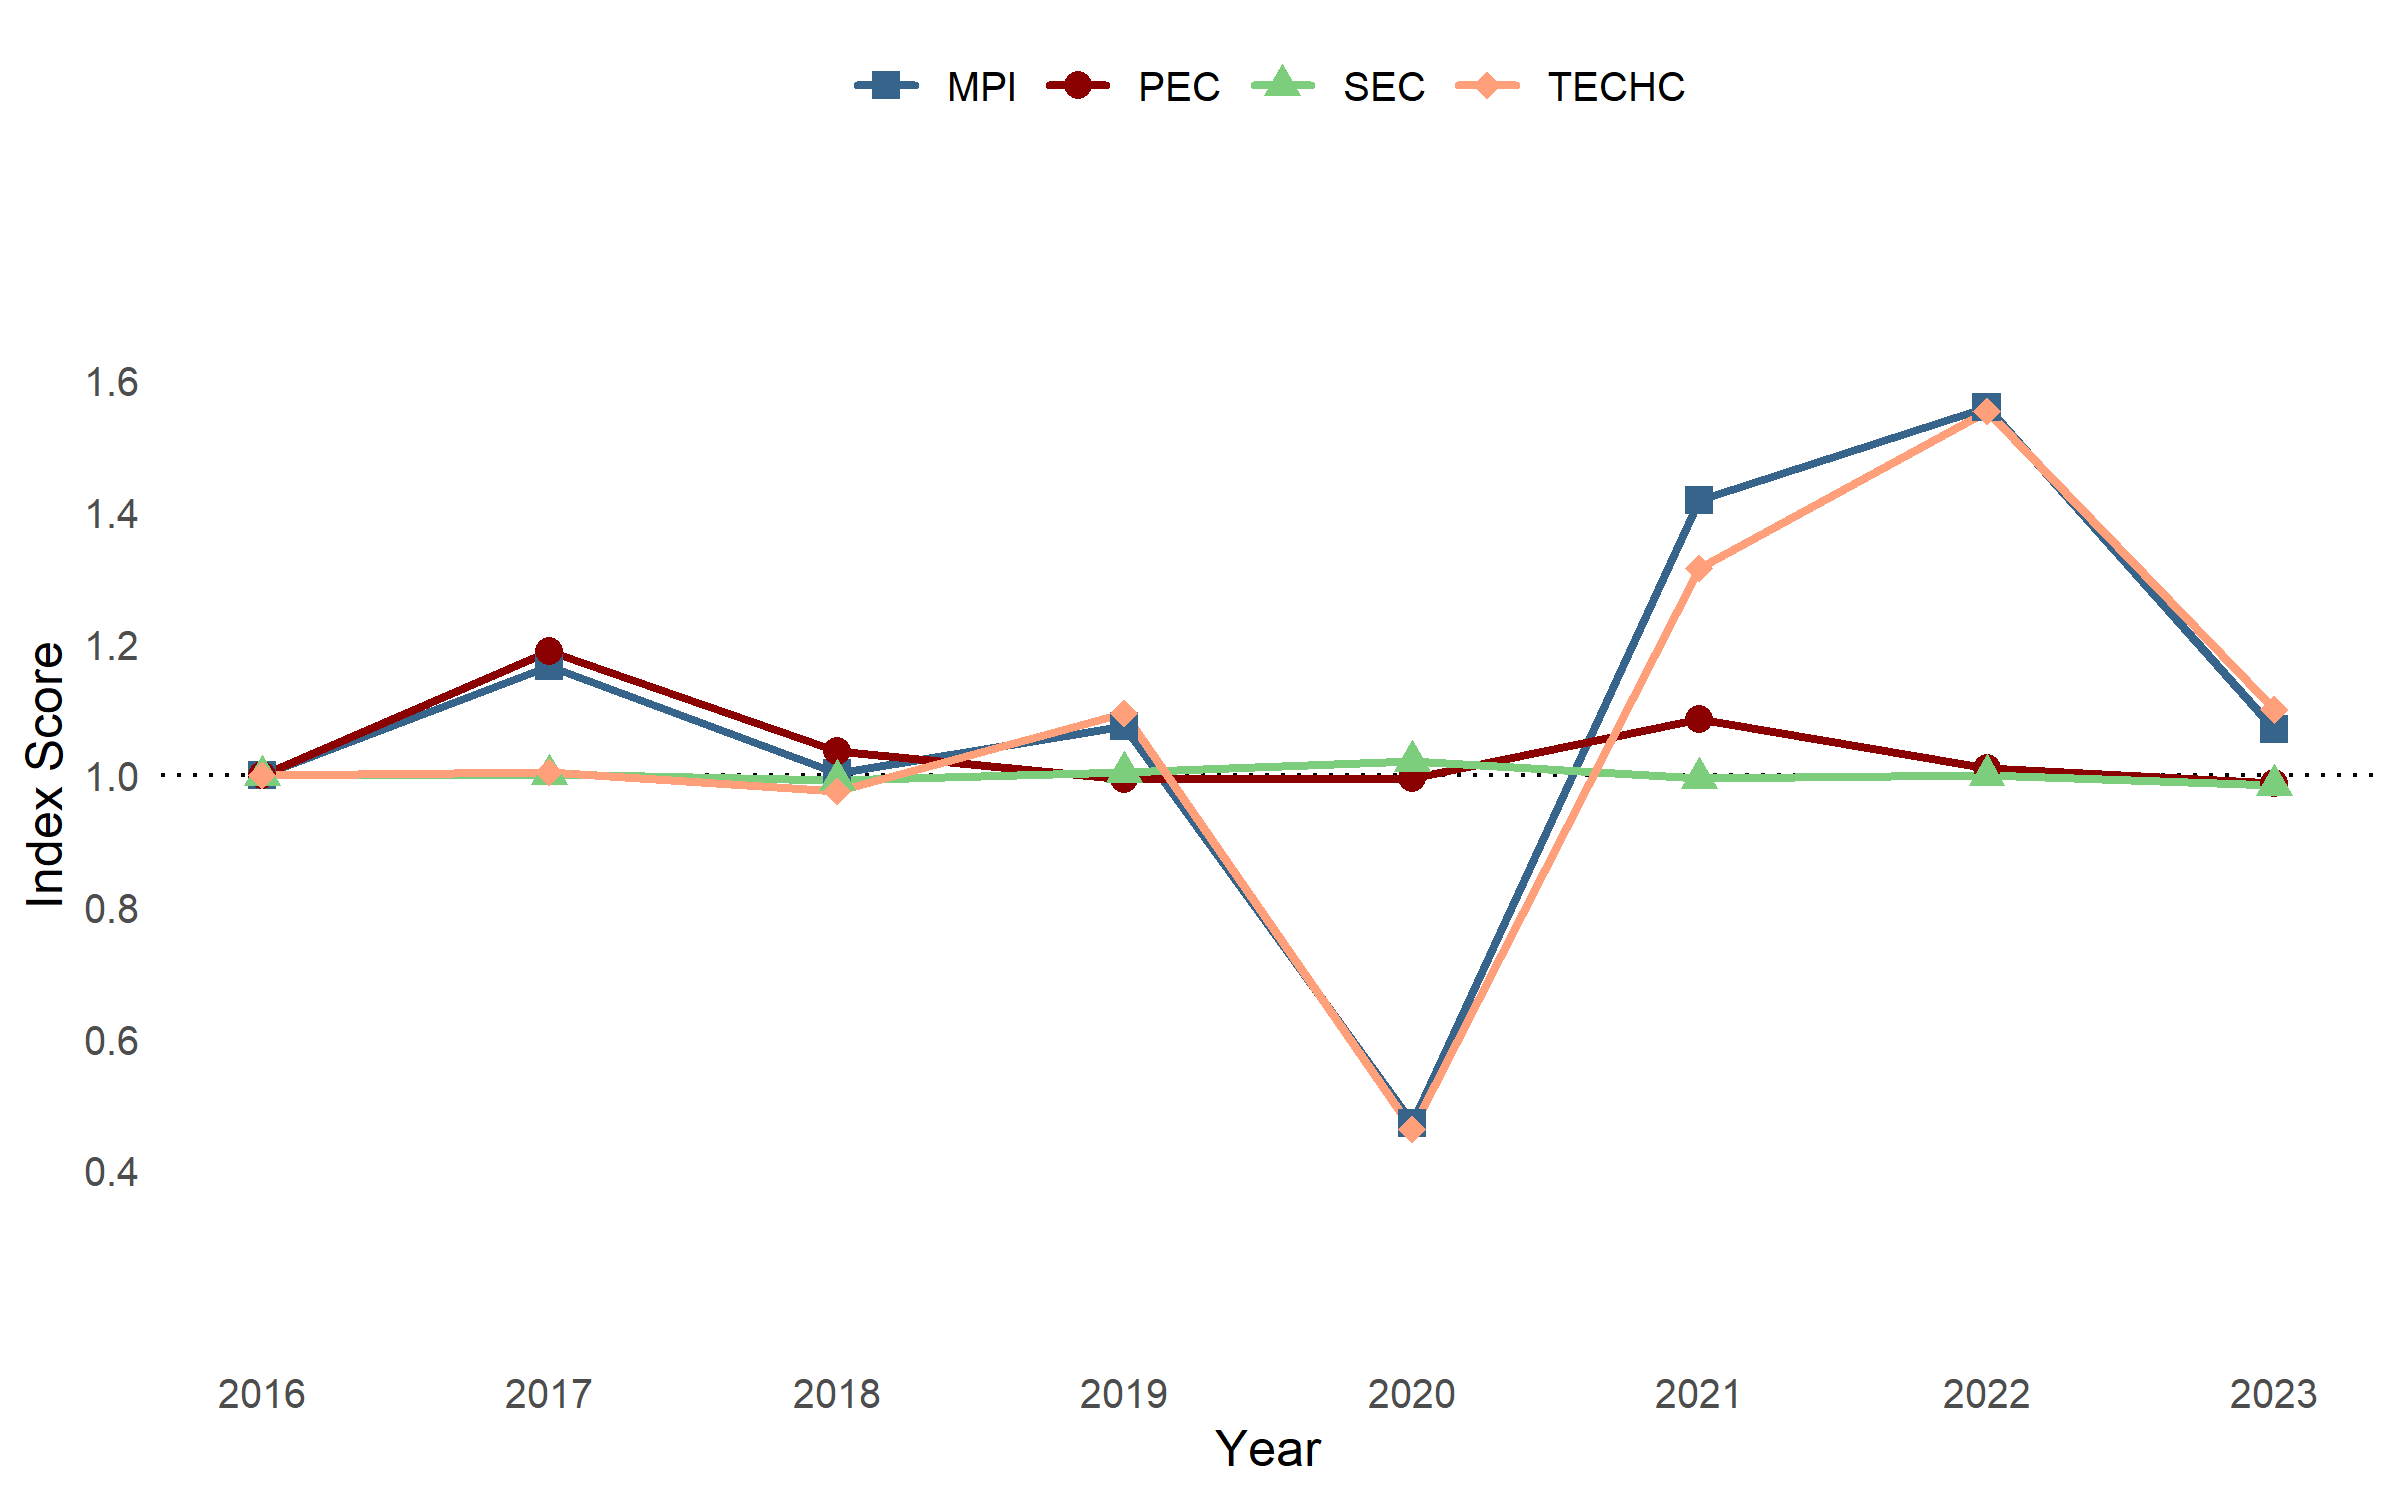
\includegraphics[width=8.2cm]{images/malmquist_plot.png}
  \vspace{-0.5cm}
  \caption{Average of Malmquist Productivity Index (MPI) and its components for each year}
  \label{fig:malmquist}
\end{figure}
\vspace{-0.5cm}

Analyzing \figref{fig:malmquist}, it is possible to observe that the average MPI was above 1 in all years, except
for 2020. The overall trend for each component of the MPI can also be examined. TECHC represented
the principal contributor for MPI fluctuations, while PEC and SEC showed a more constant evolution,
with SEC remaining almost unchanged through the whole period and being the only component with an
average value below 1. In the first years, the MPI had two years with different growth patterns. In 2017, the MPI reached a
value of 1.1657 associated with an improvement in PEC, while TECHC remained practically constant.
However in 2019, MPI growth, with a value of 1.0748, was mainly driven by an increase in TECHC.
From 2019 to 2020, an expected decline in TECHC caused the MPI to drop to a value of 0.4719, the
lowest in the period. However, observing the subsequent years it can be concluded that the Iberian
airports managed to recover well from the severe impact caused by the COVID-19, which lead to a
positive average of the MPI in the considered time period. It is important to note that, in 2021 both
TECHC and PEC increased, with PEC achieving its second highest score of 1.0852. A rise in TECHC
was expected, but this result in PEC indicates that, despite the challenging circumstances, airports were
able to improve their efficiency through better management of their resources.
%%%%%%%%%%%%%%%%%%%%%%%%%%%%%%%%%%%%%%%%%%%%%%%%%%%%%%%%%%%%%%%%%%%%%%

%\begin{table}[!h]
 %\begin{center}
  %  \begin{tabular}{lccc}
   %   Model           & $C_L$ & $C_D$ & $C_{M y}$ \\
    %  \hline
  %    Euler           & 0.083 & 61,652,021  & -0.110    \\
   %   Navier--Stokes  & 0.078 & 0.023 & -0.101    \\
    %  \hline
    %\end{tabular}
  %\end{center}
  %\caption[Table caption shown in TOC]{Table caption}
  %\label{table:simple}
%\end{table}


%%%%%%%%%%%%%%%%%%%%%%%%%%%%%%%%%%%%%%%%%%%%%%%%%%%%%%%%%%%%%%%%%%%%%%
% CONCLUSIONS
%%%%%%%%%%%%%%%%%%%%%%%%%%%%%%%%%%%%%%%%%%%%%%%%%%%%%%%%%%%%%%%%%%%%%%
%%%%%%%%%%%%%%%%%%%%%%%%%%%%%%%%%%%%%%%%%%%%%%%%%%%%%%%%%%%%%%%%%%%%%%
%     File: ExtendedAbstract_concl.tex                               %
%     Tex Master: ExtendedAbstract.tex                               %
%                                                                    %
%     Author: Andre Calado Marta                                     %
%     Last modified : 27 Dez 2011                                    %
%%%%%%%%%%%%%%%%%%%%%%%%%%%%%%%%%%%%%%%%%%%%%%%%%%%%%%%%%%%%%%%%%%%%%%
% The main conclusions of the study presented in short form.
%%%%%%%%%%%%%%%%%%%%%%%%%%%%%%%%%%%%%%%%%%%%%%%%%%%%%%%%%%%%%%%%%%%%%%
\clearpage
\section{Conclusions}
\label{sec:concl}
In this section, the main achievements of this work are summarized, followed by public policy reflections, and finally the main limitations and suggestions for future work are presented.
\subsection{Achievements}

The first-stage DEA analysis revealed that, on average, Iberian airports present relatively low effi-
ciency values in the considered period, with an average bootstrapped VRS efficiency score of 0.480, which increases to 0.522 when excluding the years affected by the COVID-19 pandemic (2020 and
2021). The results also indicated that most airports are not operating at optimal scale, with a significant
number presenting increasing returns to scale, confirming that several airports operate with overcapacity. Larger airports generally achieved higher efficiencies, while smaller and medium-sized
airports tended to have lower scores. Lastly, the Portuguese airports were found to be approximately
20\% more efficient than the Spanish ones.

The second-stage truncated regression provided insights into the exogenous factors influencing
Iberian airport efficiency. It demonstrated that airports located on islands, with military operations and
with a rail connection generally achieved higher efficiency scores. A higher share of cargo was also as-
sociated with increased efficiency, while the effect of the share of low-cost carrier (LCC) passengers was
inconclusive.

The second-stage truncated regression provided insights into the exogenous factors influencing
Iberian airport efficiency. It demonstrated that airports located on islands, with military operations and
with a rail connection generally achieved higher efficiency scores. A higher share of cargo was also as-
sociated with increased efficiency, while the effect of the share of low-cost carrier (LCC) passengers was
inconclusive.

\subsection{Public Policy Reflections}

Overall, the obtained results contribute to the understanding of the performance and determinants of
efficiency in Iberian airports. The Iberian airport network, mainly due to the Spanish network, is char-
acterized by a large number of underutilized airports, which negatively impacts the overall efficiency of
the system. This Spanish centralized management model, strongly relies on cross subsidies from large
airports to smaller ones, meaning that the profits from the larger airports are used to cover the losses
of the smaller ones. \cite{martin2001} and \cite{nerja2021} defended that this system further intensifies inefficiencies in the Spanish airport network. Conversely,
a different perspective defends that the actual system promotes equity and solidarity between Spanish
regions.

Prior studies, especially those published immediately before Aena’s privatization, identified persis-
tent sources of inefficiency and proposed different scenarios to mitigate them. The results obtained
in this dissertation invite policy makers and airport managers to reassess the current state of network
management model, taking those earlier proposals into account, namely, regionalize the management of underperforming airports; reallocate cargo traffic from airports operating under decreasing returns to
scale (DRS) to those operating under increasing returns to scale (IRS); and consider closing or merging airports that share catchment areas.

Portugal has a much smaller airport network, especially on the mainland, so the above suggestions
for Spain are not directly transferable, since they can be more relevant for smaller to medium airports.
However, one main reflection should be done. Portugal's network is centered around 3 main airports, Lisbon, Porto and Faro, but none of them has an intermodal rail connection inside
the terminal. In Spain, by contrast, the largest mainland airports such as Madrid Barajas, Barcelona El
Prat, and Malaga, as well as a medium sized airport like Jerez with a direct link to Seville, do have rail
inside the terminal. The absence of rail connections in the main Portuguese airports limits the catchment
area of those airports, and consequently their potential passengers, efficiency and growth. One can argue that the central train stations of those cities are relatively close to the airports and
only one transfer away. However, this indirect connectivity introduces inconveniences that not only in-
crease travel time but also reshape passenger behaviour. Passengers relying on indirect connections,
driven by the higher degree of uncertainty, tend to arrive earlier at the airport to avoid the risk of delays
during the transfer, which can contribute for a higher concentration of passengers and consequently the
need for larger terminal facilities. Moreover,
the inconvenience of indirect connections can discourage passengers from using rail or public trans-
port entirely, particularly when traveling with luggage. Instead, passengers may opt for private cars or
taxis, which requires better and larger parking infrastructures, at the expense of space and capital that
could otherwise support aeronautical or commercial functions.

The plan for the implementation of the new high-speed rail (HSR) line in Portugal, already contem-
plates the integration of Lisbon and Porto airports with future HSR stations (Infraestruturas de Portugal,
2025). The present study serves as evidence of the importance of this type of intermodal connections
for airport efficiency, and supports the decision of including those connections in the HSR Portugal’s
project.

Portugal operates its 10 main airports through ANA - Aeroportos de Portugal, a private company
owned by VINCI Airports, while the Spanish airport network comprises 46 airports managed by Aena, a
publicly owned company. Even though the Spanish airport network is much larger than Portugal’s, due
to the countries proximity and as both operate under centralized management models, it is important to
continuously benchmark the performance of Portuguese airports against the Spanish ones and follow
the evolution of the Spanish network closely.

Portugal’s concession agreement includes a 75 km exclusivity radius, within which new airports
cannot be developed without ANA’s consent. Outside this radius, airports may be developed indepen-
dently of the concession framework. Consequently, lessons from Spanish airports managed outside
the centralized network can offer useful insights into how those airports perform and how they affect
the efficiency of airports in the network, as certain developments can be analogous to the Portuguese
context.

This specific context makes Castell ´on Airport a particularly relevant case study. Located about one
hour north of Valencia, approximately 100 km away, Castell ´on airport is managed by the Valencian
regional government (Generalitat Valenciana) outside the Aena network. With Valencia airport operating near its maximum capacity, Generalitat Valenciana managed to
attract LCCs such as Ryanair, Volotea, and Wizz Air to Castell ´on, which have been operating regular
flights to several European destinations. Monitoring cases like Castell ´on Airport can provide insights
into how increasing the decision-making autonomy of regional airports and allowing them to negotiate
directly with airlines can help absorb unserved demand from congested airports.

\subsection{Main Limitations and Future Work}
As any research work, this dissertation has some limitations that should be acknowledged by the
readers. Firstly, the DEA methodology, being a measure of relative efficiency, depends on the sample
of DMUs under analysis. Also, the choice of inputs and outputs can significantly influence the results,
since the efficiency scores are based only on the selected variables. Lack of availability of financial
data poses one of the main limitations of this study, since only technical efficiency could be assessed. For the Portuguese airports, only data regarding the 5 of the 10 ANA airports was
available, which limits the conclusions that can be drawn about the efficiency of the entire Portuguese
airport network. Regarding the explanatory variables, the share of LCC passengers was limited to the LCCs ranked
among the top 10 airlines at each airport, which may not fully capture the impact of LCCs on airport
efficiency.

Building on the present work, the following suggestions are made to address some of the limitations
mentioned in the previous section and to further develop the topic. As DEA measures relative efficiency, increasing the sample size by including more airports, espe-
cially the remaining Portuguese airports managed by ANA, or even expanding the analysis to include
airports from other countries, would improve the robustness of the results and provide a wider bench-
mark comparison. Additionally, future Iberian studies could aim to include financial data, to assess cost
efficiency in addition to technical efficiency. As a continuation of the present work, the same methodology can be applied for the subsequent
years, i.e, from 2024 onwards, in order to continuously monitor the efficiency of the Iberian airport
networks.

%%%%%%%%%%%%%%%%%%%%%%%%%%%%%%%%%%%%%%%%%%%%%%%%%%%%%%%%%%%%%%%%%%%%%%
% ACKNOWLEDGMENTS
%%%%%%%%%%%%%%%%%%%%%%%%%%%%%%%%%%%%%%%%%%%%%%%%%%%%%%%%%%%%%%%%%%%%%%
%%%%%%%%%%%%%%%%%%%%%%%%%%%%%%%%%%%%%%%%%%%%%%%%%%%%%%%%%%%%%%%%%%%%%%
%     File: ExtendedAbstract_ackno.tex                               %
%     Tex Master: ExtendedAbstract.tex                               %
%                                                                    %
%     Author: Andre Calado Marta                                     %
%     Last modified : 27 Dez 2011                                    %
%%%%%%%%%%%%%%%%%%%%%%%%%%%%%%%%%%%%%%%%%%%%%%%%%%%%%%%%%%%%%%%%%%%%%%
% Acknowledge persons and institutions that supported this work.
%%%%%%%%%%%%%%%%%%%%%%%%%%%%%%%%%%%%%%%%%%%%%%%%%%%%%%%%%%%%%%%%%%%%%%

\section*{Acknowledgements}

The author would like to thank ...



%%%%%%%%%%%%%%%%%%%%%%%%%%%%%%%%%%%%%%%%%%%%%%%%%%%%%%%%%%%%%%%%%%%%%%
% REFERENCES
%%%%%%%%%%%%%%%%%%%%%%%%%%%%%%%%%%%%%%%%%%%%%%%%%%%%%%%%%%%%%%%%%%%%%%

% Produces the bibliography section when processed by BibTeX
%
% Bibliography style
% > entries ordered alphabetically
%\bibliographystyle{plain}
% > unsorted with entries appearing in the order in which the citations appear.
\bibliographystyle{unsrt}
% > entries ordered alphabetically, with first names and names of journals and months abbreviated
%\bibliographystyle{abbrv}
% > entries ordered alphabetically, with reference markers based on authors' initials and publication year
%\bibliographystyle{alpha}

% External bibliography database file in the BibTeX format (ExtendedAbstract_ref_db.bib)
\bibliography{ExtendedAbstract_ref_db}

%%%%%%%%%%%%%%%%%%%%%%%%%%%%%%%%%%%%%%%%%%%%%%%%%%%%%%%%%%%%%%%%%%%%%%
\end{document}
%%%%%%%%%%%%%%%%%%%%%%%%%%%%%%%%%%%%%%%%%%%%%%%%%%%%%%%%%%%%%%%%%%%%%%

